\documentclass[11pt,a4paper]{article}

% ---------------------------------------------------------------
% Packages
% ---------------------------------------------------------------
\usepackage[utf8]{inputenc}
\usepackage[T1]{fontenc}
\usepackage{lmodern}
\usepackage[margin=1in]{geometry}
\usepackage{amsmath,amssymb}
\usepackage{booktabs}
\usepackage{array}
\usepackage{graphicx}
\usepackage{microtype}
\usepackage{enumitem}
\usepackage{xcolor}
\usepackage{tikz}
\usetikzlibrary{shapes.geometric,arrows.meta,positioning,calc,fit}
\usepackage[hidelinks]{hyperref}

% ---------------------------------------------------------------
% Macros
% ---------------------------------------------------------------
\newcommand{\lo}[1]{\underline{#1}}
\newcommand{\up}[1]{\overline{#1}}
\newcommand{\credal}{\mathcal{C}}
\newcommand{\simplex}{\Delta_K}
\newcommand{\TV}{\mathrm{TV}}
\newcommand{\TU}{\mathrm{TU}}
\newcommand{\AU}{\mathrm{AU}}
\newcommand{\EU}{\mathrm{EU}}
\newcommand{\ND}{\mathrm{ND}}

% TikZ styles
\tikzset{
  block/.style={rectangle, draw, rounded corners=2pt, align=center,
                minimum height=1.0cm, text width=3.6cm, font=\small, fill=gray!8},
  wide/.style={rectangle, draw, rounded corners=2pt, align=center,
               minimum height=1.0cm, text width=7.8cm, font=\small, fill=gray!8},
  data/.style={rectangle, draw, align=center, minimum height=0.9cm,
               text width=3.6cm, font=\small, fill=blue!6},
  decision/.style={diamond, draw, aspect=2.2, align=center, font=\small,
                   inner sep=1pt, fill=yellow!15},
  out/.style={rectangle, draw, rounded corners=2pt, align=center,
              minimum height=0.9cm, text width=3.0cm, font=\small, fill=green!10},
  arrow/.style={-{Latex[length=2.5mm]}, thick}
}

\title{Credal Uncertainty Quantification for Reliable Stance Detection on Unseen Targets}
\author{}
\date{}

\begin{document}

\maketitle
\vspace{-3em}

\begin{abstract}
\noindent
Stance detection identifies whether the author of a text is in favor of, against, or
neutral towards a given target. Current models output a single probability distribution
over stance labels. That one distribution mixes up aleatoric uncertainty (the text is
genuinely ambiguous and humans disagree about it) with epistemic uncertainty (the model has
never seen this target or domain). As a result, stance detectors are over-confident on
unseen targets and cannot give a principled reason to abstain. This project proposes a
stance detector that outputs a credal set, i.e.\ a convex set of probability
distributions, summarised as a lower and an upper probability for each stance. The credal
set is built from a diverse ensemble of transformer and LLM backbones, decomposed into
aleatoric and epistemic parts using upper and lower entropy, calibrated with conformal
prediction to obtain a coverage guarantee, and turned into a decision (predict, return a
set of plausible stances, or defer to a human) with imprecise-probability decision rules.
No new annotation is collected: human label distributions come from the publicly released
raw annotator labels of SemEval-2016. The method is evaluated in in-target, cross-target
and zero-shot settings against seven families of uncertainty baselines. To our knowledge,
this is the first application of credal uncertainty quantification to stance detection.
\end{abstract}

\tableofcontents
\newpage

% ===============================================================
\section{Introduction and Motivation}
% ===============================================================

\textbf{Stance detection} takes a piece of text and a \emph{target} (a person, policy,
product or claim) and decides whether the author is \textsc{favor}, \textsc{against} or
\textsc{none} towards that target~\cite{mohammad2016,kucuk2020,survey2024}. It is used in
misinformation analysis, content moderation, political opinion tracking and argument
mining.

A stance detector is normally a classifier that returns one probability vector, for
example $p = [0.44, 0.41, 0.15]$ over $\{\textsc{favor}, \textsc{against}, \textsc{none}\}$.
That one vector cannot distinguish two very different situations:

\begin{enumerate}[leftmargin=*]
  \item \textbf{Ambiguity (aleatoric uncertainty).} The text itself is unclear. Example:
  \emph{``Oh great, another `climate emergency' summit. I'm sure the private jets will fix
  it.''} Is the author for or against climate action? Even human annotators split on this.
  The VAST benchmark reports a Krippendorff's $\alpha$ of only $0.427$~\cite{allaway2020}.
  No amount of extra training data will remove this uncertainty, because it lives in the
  text.

  \item \textbf{Ignorance (epistemic uncertainty).} The model lacks knowledge. Example: a
  tweet about the target \emph{``Digital euro''} when the model was trained on tweets about
  abortion, feminism and atheism. More data about the new target \emph{would} remove this
  uncertainty.
\end{enumerate}

Both situations can produce the same output vector. In the first case the right action is
to flag the text as contested; in the second it is to defer to a human or to collect labels
for the new target. A single probability vector gives no basis for choosing between them.
Recent analyses of LLM stance detection reach the same conclusion: hard instances are
usually ambiguous or context-dependent, and systems used in sensitive settings should report
uncertainty and allow human review~\cite{sici2026}.

This project addresses the gap with \textbf{credal sets}: instead of one distribution, the
model predicts a \emph{set} of plausible distributions. The size and shape of that set
separate ambiguity from ignorance, and imprecise-probability decision theory tells us what
to do with it.

% ===============================================================
\section{Problem Statement}
% ===============================================================

\begin{quote}
Given a text $x$ and a target $t$, existing stance detectors output a single probability
vector $p(y \mid x, t)$ over $\mathcal{Y} = \{\textsc{favor}, \textsc{against},
\textsc{none}\}$. This vector conflates (i) \emph{aleatoric} uncertainty, arising from
sarcasm, implicit stance, missing context and genuine human disagreement, with (ii)
\emph{epistemic} uncertainty, arising from unseen targets, domain shift and limited data.
Consequently, models are over-confident on unseen targets and cannot justify abstention.

We propose a stance detector that outputs a \emph{credal set} $\credal(x,t) \subseteq
\simplex$ of distributions, represented by class-wise lower and upper probabilities
$[\lo{P}(y), \up{P}(y)]$, built from ensembles of transformer and LLM backbones. The system
(a) separates aleatoric from epistemic uncertainty, (b) provides a distribution-free
conformal coverage guarantee for the human label distribution, and (c) uses the credal set
to predict, return a set of plausible stances, or defer to a human. It is evaluated on
in-target, cross-target and zero-shot benchmarks, and against human label distributions
derived from existing raw multi-annotator stance data.
\end{quote}

\paragraph{Research questions.}
\begin{description}[leftmargin=1.6cm, style=nextline]
  \item[RQ1] Do credal stance models give better uncertainty estimates than standard
  methods (softmax, MC Dropout, deep ensembles, evidential deep learning), in-target and
  across targets?
  \item[RQ2] Does the credal decomposition separate ambiguity from ignorance? Does the
  epistemic part rise on unseen targets, and does the aleatoric part track human
  disagreement?
  \item[RQ3] Can we guarantee, with high probability, that the predicted set covers the true
  human label distribution?
  \item[RQ4] Does credal uncertainty lead to better decisions (abstention, deferral,
  set-valued prediction) than confidence thresholding?
  \item[RQ5] Do credal sets built from LLM ensembles beat verbalised and sampling-based LLM
  confidence?
\end{description}

\paragraph{Scope.} The claim is about \emph{reliability}, not about a new state-of-the-art
macro-F1. The system classifies texts, never the beliefs of identifiable people.

% ===============================================================
\section{Background}
% ===============================================================

\subsection{Credal sets}

Let $K = 3$ and let $\simplex$ be the probability simplex. A \textbf{credal set} is a closed
convex set $\credal \subseteq \simplex$ of candidate distributions for an imprecisely known
ground truth~\cite{walley1991}. We use \emph{probability-interval} credal sets, defined by
lower bounds $l$ and upper bounds $u$ per class:
\begin{equation}
  \credal(l,u) = \{\, p \in \simplex : l_k \le p_k \le u_k \ \text{for all } k \,\}.
  \label{eq:credal}
\end{equation}
The lower and upper probabilities are $\lo{P}(k) = \min_{p \in \credal} p_k$ and
$\up{P}(k) = \max_{p \in \credal} p_k$.

Figure~\ref{fig:simplex} shows why a credal set carries two kinds of information. A
\emph{small} set centred on a spread-out distribution means the model is sure \emph{that} the
text is ambiguous (aleatoric). A \emph{large} set means the model does not know which
distribution is right (epistemic).

\begin{figure}[t]
\centering
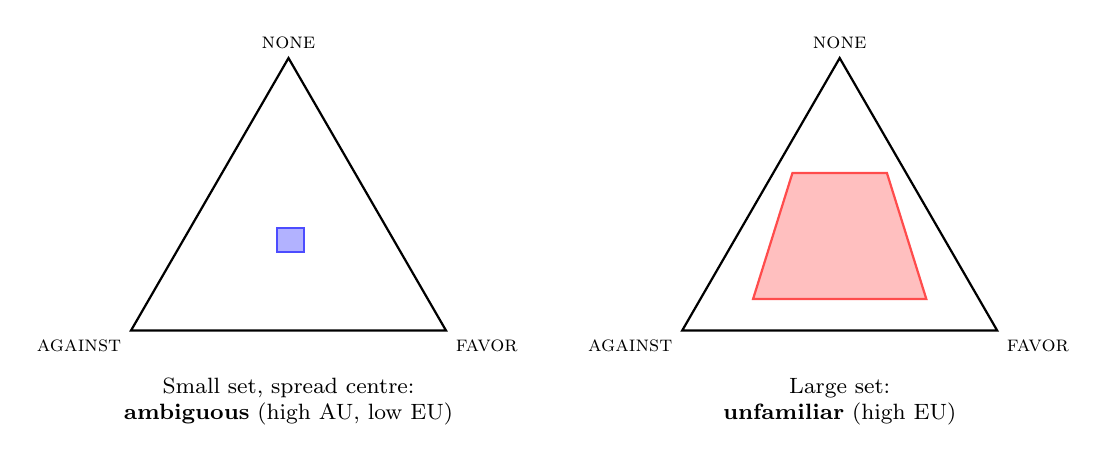
\begin{tikzpicture}[scale=1.0]
  % ---- left simplex: ambiguous but known ----
  \begin{scope}[shift={(0,0)}]
    \coordinate (A) at (0,0);
    \coordinate (B) at (4,0);
    \coordinate (C) at (2,3.46);
    \draw[thick] (A) -- (B) -- (C) -- cycle;
    \node[below left, font=\footnotesize] at (A) {\textsc{against}};
    \node[below right, font=\footnotesize] at (B) {\textsc{favor}};
    \node[above, font=\footnotesize] at (C) {\textsc{none}};
    \fill[blue!30, draw=blue!70, thick] (1.85,1.0) -- (2.2,1.0) -- (2.2,1.3) -- (1.85,1.3) -- cycle;
    \node[font=\footnotesize, align=center] at (2,-0.9) {Small set, spread centre:\\\textbf{ambiguous} (high AU, low EU)};
  \end{scope}
  % ---- right simplex: unknown ----
  \begin{scope}[shift={(7,0)}]
    \coordinate (A) at (0,0);
    \coordinate (B) at (4,0);
    \coordinate (C) at (2,3.46);
    \draw[thick] (A) -- (B) -- (C) -- cycle;
    \node[below left, font=\footnotesize] at (A) {\textsc{against}};
    \node[below right, font=\footnotesize] at (B) {\textsc{favor}};
    \node[above, font=\footnotesize] at (C) {\textsc{none}};
    \fill[red!25, draw=red!70, thick] (0.9,0.4) -- (3.1,0.4) -- (2.6,2.0) -- (1.4,2.0) -- cycle;
    \node[font=\footnotesize, align=center] at (2,-0.9) {Large set:\\\textbf{unfamiliar} (high EU)};
  \end{scope}
\end{tikzpicture}
\caption{Two credal sets on the stance simplex. Each point in a triangle is a probability
vector over the three stances. Left: the model is confident that the distribution is spread
between \textsc{favor} and \textsc{against}, i.e.\ the text is contested. Right: the model
cannot narrow down the distribution at all, i.e.\ it has not learned this target.}
\label{fig:simplex}
\end{figure}

\subsection{Uncertainty measures on credal sets}

Following Abell\'an et al.~\cite{abellan2006} and H\"ullermeier and
Waegeman~\cite{hullermeier2021}, with $H$ the Shannon entropy in bits:
\begin{align}
  \TU(\credal) &= \up{H}(\credal) = \max_{p \in \credal} H(p) \quad\text{(total uncertainty)},\\
  \AU(\credal) &= \lo{H}(\credal) = \min_{p \in \credal} H(p) \quad\text{(aleatoric)},\\
  \EU(\credal) &= \up{H}(\credal) - \lo{H}(\credal) \quad\text{(epistemic)}.
\end{align}
For $K=3$ the maximum entropy is $\log_2 3 \approx 1.585$ bits. Sale et
al.~\cite{sale2023} show that the \emph{volume} of a credal set is a sound epistemic measure
only in the binary case, which is why we use the entropy decomposition for three classes.

\subsection{Classical versus modern credal models}

A frequent objection is that ``credal networks only work on tabular data''. This is true of
\emph{classical} credal networks~\cite{cozman2000} and the Naive Credal
Classifier~\cite{corani2008}: they place imprecise probability tables \emph{inside} a
graphical model over discrete variables, and exact inference is intractable for more than a
handful of such variables. One cannot build a credal network over a 30{,}000-word
vocabulary.

Modern \emph{credal deep learning} is different (Table~\ref{tab:classical}). The credal set
lives at the \emph{output} of a neural network, as lower and upper class probabilities. The
raw input, whether image, text or graph, is handled by an ordinary encoder; the credal
construction only ever sees probability vectors. Published evidence on language data
includes credal sets on the ChaosNLI natural-language-inference
benchmark~\cite{javanmardi2024,hofman2026}, credal LLMs built from LoRA
ensembles~\cite{manchingal2026}, and a credal attention mechanism inside the Transformer
itself~\cite{credaltransformer2025}. Stance detection has the same structure as NLI (a
text pair and three classes), and EZ-Stance even reformulates zero-shot stance detection
\emph{as} NLI~\cite{zhao2024}. The machinery therefore carries over directly.

\begin{table}[t]
\centering
\small
\begin{tabular}{p{3.2cm} p{5.2cm} p{5.6cm}}
\toprule
& Classical credal models & Modern credal deep learning \\
\midrule
Examples & Credal networks~\cite{cozman2000}, Naive Credal Classifier~\cite{corani2008} &
  Credal Wrapper~\cite{wang2025wrapper}, Credal Deep Ensembles~\cite{wang2024crede},
  CreINNs~\cite{wang2025creinn}, conformal credal sets~\cite{javanmardi2024},
  credal LLMs~\cite{manchingal2026} \\
Where the credal set lives & Inside the model (imprecise conditional probability tables) &
  At the output (lower/upper class probabilities) \\
Input data & Discrete, tabular & Any: images, text, graphs, LLM tokens \\
Why & Exact inference needs few discrete variables & The encoder handles the raw input \\
\bottomrule
\end{tabular}
\caption{The two meanings of ``credal'' in machine learning. This project uses the modern
kind; a classical credal network appears only as an optional interpretability module
(Section~\ref{sec:m9}).}
\label{tab:classical}
\end{table}

% ===============================================================
\section{Related Work and Research Gap}
% ===============================================================

\paragraph{Stance detection.} Benchmarks include SemEval-2016~\cite{mohammad2016} (five
targets, tweets), VAST~\cite{allaway2020} (thousands of zero-shot topics) and
EZ-Stance~\cite{zhao2024} (47k pairs, target- and domain-based zero-shot subtasks). LLM
stance detection suffers from sentiment--stance spurious correlations and target bias;
FACTUAL~\cite{factual2024} corrects this with a calibration network, but still outputs a
single distribution.

\paragraph{Uncertainty in NLP.} Deep ensembles~\cite{lakshminarayanan2017}, MC
Dropout~\cite{gal2016}, evidential deep learning~\cite{sensoy2018} and conformal
prediction~\cite{angelopoulos2023} are the standard tools. Human label variation is
increasingly treated as signal rather than noise~\cite{plank2022,uma2021}; ChaosNLI collects
about 100 annotations per NLI item~\cite{nie2020}, and multi-perspective stance detection
trains on individual annotator labels~\cite{muscato2024}.

\paragraph{Credal deep learning.} The Credal Wrapper~\cite{wang2025wrapper} builds a credal
set from any ensemble post hoc; Credal Deep Ensembles~\cite{wang2024crede} and
CreINNs~\cite{wang2025creinn} train networks to output intervals directly; conformalized
credal set predictors~\cite{javanmardi2024} add coverage guarantees; EffCre~\cite{hofman2026}
obtains credal sets from a single model; credal LLMs~\cite{manchingal2026} use LoRA
ensembles. Decision making with credal sets uses interval dominance and related
rules~\cite{troffaes2007}, and credal classifiers are evaluated with utility-discounted
accuracy~\cite{zaffalon2012}.

\paragraph{Gap.} A literature search (October 2026) found no published work that applies
credal sets or imprecise probabilities to stance detection. The closest work is on NLI. The
combination of (i) credal uncertainty decomposition, (ii) conformal guarantees for the human
label distribution and (iii) imprecise-probability decision rules has not been studied for
stance.

% ===============================================================
\section{Proposed Solution: System Architecture}
% ===============================================================

Figure~\ref{fig:arch} shows the end-to-end pipeline. Text and target enter a diverse
ensemble; the ensemble's $M$ probability vectors are turned into a credal set; the credal
set is decomposed into aleatoric and epistemic uncertainty, calibrated with conformal
prediction, and converted into a decision.

\begin{figure}[p]
\centering
\begin{tikzpicture}[node distance=0.55cm and 0.9cm]
  % Row 1: data
  \node[data] (bench) {M1: Benchmarks\\SemEval-16, VAST,\\EZ-Stance};
  \node[data, right=of bench] (hlv) {M2: Human label\\distributions\\(SemEval-16 raw labels)};
  % Row 2: encoding
  \node[block, below=of bench] (enc) {M3: Input encoding\\\texttt{[target] [SEP] [text]}\\or LLM prompt};
  % Row 3: ensembles
  \node[block, below=of enc] (ensA) {M4a: DeBERTa-v3\\ensemble ($M=8$)};
  \node[block, right=of ensA] (ensB) {M4b: LLM + 8 LoRA\\adapters};
  \coordinate (midEns) at ($(ensA.south)!0.5!(ensB.south)$);
  % Row 4: credal layer
  \node[wide, below=0.9cm of midEns] (credal)
    {M5: Credal layer\\$l_k=\min_m p_{m,k}$,\quad $u_k=\max_m p_{m,k}$,\quad
     intersection probability $p^{*}$};
  % Row 5: decomposition + conformal
  \node[block, below left=0.8cm and 0.4cm of credal.south] (dec)
    {M6: Decomposition\\$\TU=\up{H}$, $\AU=\lo{H}$,\\$\EU=\up{H}-\lo{H}$};
  \node[block, below right=0.8cm and 0.4cm of credal.south] (conf)
    {M7: Conformal\\calibration\\radius $\hat q$, coverage $1-\alpha$};
  \coordinate (midDC) at ($(dec.south)!0.5!(conf.south)$);
  % Row 6: decision
  \node[wide, below=0.9cm of midDC] (route)
    {M8: Decision and routing\\interval dominance $\rightarrow$
     \{\,predict, set-valued, defer\,\}};
  % Row 7: outputs
  \node[out, below left=0.8cm and 1.9cm of route.south] (o1) {Single stance};
  \node[out, below=0.8cm of route.south] (o2) {Set of plausible\\stances};
  \node[out, below right=0.8cm and 1.9cm of route.south] (o3) {Defer to human};
  % Arrows
  \draw[arrow] (bench) -- (enc);
  \draw[arrow] (enc) -- (ensA);
  \draw[arrow] (enc.east) -| (ensB.north);
  \draw[arrow] (ensA.south) -- ++(0,-0.4) -| (credal.north);
  \draw[arrow] (ensB.south) -- ++(0,-0.4) -| (credal.north);
  \draw[arrow] (credal.south) -- ++(0,-0.35) -| (dec.north);
  \draw[arrow] (credal.south) -- ++(0,-0.35) -| (conf.north);
  \draw[arrow] (hlv.east) -- ++(0.7,0) |- node[pos=0.25, right, font=\scriptsize] {$\lambda_x$ (human label distribution)} (conf.east);
  \draw[arrow] (dec.south) -- ++(0,-0.35) -| (route.north);
  \draw[arrow] (conf.south) -- ++(0,-0.35) -| (route.north);
  \draw[arrow] (route.south) -- ++(0,-0.3) -| (o1.north);
  \draw[arrow] (route.south) -- (o2.north);
  \draw[arrow] (route.south) -- ++(0,-0.3) -| (o3.north);
  % label on the ensemble -> credal edge
  \node[font=\scriptsize, above] at ($(midEns)+(0,-0.4)$) {$M$ probability vectors $p_1,\dots,p_M$};
\end{tikzpicture}
\caption{End-to-end architecture. M1--M8 are the modules described in
Sections~\ref{sec:m1}--\ref{sec:m8}. Human label distributions enter only at calibration
and evaluation time; no module is trained on them except in one ablation.}
\label{fig:arch}
\end{figure}

% ---------------------------------------------------------------
\subsection{M1: Data layer}\label{sec:m1}
% ---------------------------------------------------------------

Table~\ref{tab:data} lists the benchmarks and their roles. All sources are mapped to a
unified label set $\{\textsc{favor}=0, \textsc{against}=1, \textsc{none}=2\}$.

\begin{table}[ht]
\centering
\small
\begin{tabular}{l l p{3.4cm} p{4.4cm}}
\toprule
Dataset & Domain & Targets & Role \\
\midrule
SemEval-2016 Task 6~\cite{mohammad2016} & Tweets & 5 fixed targets & In-target, leave-one-target-out \\
VAST~\cite{allaway2020} & NYT comments & $\sim$5{,}600 topics & Zero-shot \\
EZ-Stance~\cite{zhao2024} & Tweets & Noun-phrase + claim targets & Zero-shot (target- and domain-based) \\
ChaosNLI~\cite{nie2020} & NLI & -- & Secondary conformal check (100 annotators/item) \\
\bottomrule
\end{tabular}
\caption{Datasets. Sizes should be verified against the official releases; tweet
datasets are distributed as IDs and some tweets are no longer retrievable.}
\label{tab:data}
\end{table}

\paragraph{Evaluation splits.}
\begin{itemize}[leftmargin=*]
  \item \textbf{In-target}: official SemEval train/test split.
  \item \textbf{Leave-one-target-out (LOTO)}: train on four SemEval targets, test on the
  fifth; five folds. A controlled epistemic shift.
  \item \textbf{Zero-shot}: VAST and EZ-Stance official zero-shot test sets. A strong
  epistemic shift.
  \item \textbf{Seen/unseen pool}: in-target test items (label $0$) mixed with zero-shot test
  items (label $1$), for unseen-target detection.
\end{itemize}

% ---------------------------------------------------------------
\subsection{M2: Human label distributions from existing raw annotations}\label{sec:m2}
% ---------------------------------------------------------------

The project collects \textbf{no new annotations}. SemEval-2016 publicly releases every
crowd worker's individual stance label for each tweet~\cite{mohammad2016,mohammad2017}. We
inspected the released file (October 2026); its contents are summarised in
Table~\ref{tab:raw}.

\begin{table}[ht]
\centering
\small
\begin{tabular}{p{5.4cm} r p{6.4cm}}
\toprule
Subset & Count & Note \\
\midrule
Shared-task tweets with all votes & 4{,}306 & median 8 annotators per tweet \\
Low-agreement tweets (dropped from the task, agreement $<60\%$) & 1{,}385 & mean label entropy 1.445 bits (max 1.585) \\
Targets covered & 5 & Atheism, Feminist Movement, Hillary Clinton, Legalization of Abortion, Donald Trump \\
\bottomrule
\end{tabular}
\caption{Contents of the SemEval-2016 raw stance annotation file.}
\label{tab:raw}
\end{table}

For each tweet $x$ with $n$ votes we compute the empirical human label distribution and
its entropy:
\begin{equation}
  \lambda_x = \frac{(n_{\textsc{favor}},\, n_{\textsc{against}},\, n_{\textsc{none}})}{n},
  \qquad
  H(\lambda_x) = -\sum_k \lambda_{x,k} \log_2 \lambda_{x,k}.
\end{equation}
The raw \textsc{neutral} answer is mapped to \textsc{none}, matching the official label
derivation. Because $n \approx 8$ is small, we also report a Dirichlet-smoothed version
$(n_k + 0.5)/(n + 1.5)$ and repeat the conformal analysis on the $n \ge 10$ subset.

From this file we build five human-grounded splits:
\begin{description}[leftmargin=2.3cm, style=nextline]
  \item[HLV-train] official SemEval train tweets minus HLV-cal (member training).
  \item[HLV-cal] 20\% of the train tweets, stratified by target and held out from training
  (conformal calibration).
  \item[HLV-test] official SemEval test tweets with raw votes (human-alignment and coverage
  evaluation).
  \item[HLV-unseen] every tweet about one target (e.g.\ \emph{Donald Trump}) that is
  excluded from training (human-labelled unseen-target test).
  \item[HLV-ambig] the 1{,}385 low-agreement tweets (ambiguity stress test; AU should be
  high here, and EU should \emph{not} be driven by it).
\end{description}

% ---------------------------------------------------------------
\subsection{M3: Input encoding}\label{sec:m3}
% ---------------------------------------------------------------

\textbf{Encoder path.} Sentence-pair input with the target first so it is never truncated:
\begin{center}
\texttt{[CLS] Climate Change is a Real Concern [SEP] We need to act NOW. \#ClimateAction [SEP]}
\end{center}

\textbf{LLM path.} An instruction prompt (\emph{``Target: \dots\ Text: \dots\ What is the
author's stance towards the target? Answer with exactly one word: favor, against, or
none.''}) followed by a \emph{verbalizer readout}: the next-token logits of the three answer
words are passed through a softmax restricted to those three tokens. This yields a proper
3-class probability vector with no free-text generation and no parsing errors.

% ---------------------------------------------------------------
\subsection{M4: Backbone ensembles}\label{sec:m4}
% ---------------------------------------------------------------

The credal set is only as informative as the ensemble is diverse, so diversity is
engineered explicitly.

\begin{table}[ht]
\centering
\small
\begin{tabular}{l p{5.3cm} p{5.3cm}}
\toprule
& Path A: encoder ensemble & Path B: LLM LoRA ensemble \\
\midrule
Backbone & DeBERTa-v3-large~\cite{he2023} & Qwen2.5-7B-Instruct (frozen) \\
Members & $M=8$, full fine-tuning & $M=8$ LoRA adapters~\cite{hu2022,wang2023lora} \\
Diversity & Different seeds; 80\% bootstrap of training data per member &
  Seeds; 80\% bootstrap; two instruction paraphrases \\
Loss & Cross-entropy on hard labels & Cross-entropy on the 3-token restricted softmax \\
Optimiser & AdamW, lr $10^{-5}$, 6 epochs, early stopping & AdamW, lr $10^{-4}$, cosine, 2 epochs \\
\bottomrule
\end{tabular}
\caption{The two backbone paths. Member logits are cached to disk once, so all credal,
conformal and decision experiments run on CPU in seconds.}
\label{tab:ens}
\end{table}

The output of M4 for an input $(x,t)$ is a matrix $P \in \mathbb{R}^{M \times K}$ whose row
$m$ is $p_m = \mathrm{softmax}(f_m(x,t))$.

% ---------------------------------------------------------------
\subsection{M5: Credal layer}\label{sec:m5}
% ---------------------------------------------------------------

\textbf{Construction (Credal Wrapper~\cite{wang2025wrapper}).} From the $M$ member
distributions take the class-wise extremes:
\begin{equation}
  l_k = \min_{m} p_{m,k}, \qquad u_k = \max_{m} p_{m,k}, \qquad
  \credal(x) = \{p \in \simplex : l \le p \le u\}.
  \label{eq:bounds}
\end{equation}
Each bound is attained by some member and every member lies in $\credal(x)$, so the bounds
are reachable and no tightening step is needed.

\textbf{Point prediction (intersection probability~\cite{wang2025wrapper}).} For metrics
that need one distribution:
\begin{equation}
  \alpha = \frac{1 - \sum_k l_k}{\sum_k (u_k - l_k)}, \qquad
  p^{*}_k = l_k + \alpha\,(u_k - l_k), \qquad \hat y = \arg\max_k p^{*}_k.
  \label{eq:ip}
\end{equation}

\textbf{Alternatives compared in ablation.} Credal sets from MC-Dropout samples; Credal Deep
Ensembles, which train each network to output intervals directly~\cite{wang2024crede};
CreINNs~\cite{wang2025creinn}; EffCre, which needs only a single model~\cite{hofman2026};
and credal ensemble distillation into one student~\cite{credaldistill2025}.

% ---------------------------------------------------------------
\subsection{M6: Uncertainty decomposition}\label{sec:m6}
% ---------------------------------------------------------------

\textbf{Upper entropy} $\up{H}$ is a concave maximisation over a box-constrained simplex.
From the KKT conditions the maximiser is $p_k = \mathrm{clip}(\tau, l_k, u_k)$ for a scalar
$\tau$ found by bisection so that $\sum_k p_k = 1$ (``water-filling'').

\textbf{Lower entropy} $\lo{H}$: entropy is concave, so its minimum over the polytope is
attained at a vertex. For $K=3$ there are at most 12 candidate vertices, which are
enumerated directly.

\textbf{Epistemic uncertainty} is then $\EU = \up{H} - \lo{H}$. Table~\ref{tab:interp}
gives the interpretation.

\begin{table}[ht]
\centering
\small
\begin{tabular}{c c l l}
\toprule
AU & EU & Meaning & Typical cause \\
\midrule
low & low & Confident, clear & Explicit stance on a seen target \\
high & low & Ambiguous / contested & Sarcasm, mixed stance; humans also disagree \\
any & high & Unfamiliar & Unseen target, new domain, emerging event \\
high & high & Both & Ambiguous text on an unseen target \\
\bottomrule
\end{tabular}
\caption{Reading the decomposition.}
\label{tab:interp}
\end{table}

% ---------------------------------------------------------------
\subsection{M7: Conformal credal calibration}\label{sec:m7}
% ---------------------------------------------------------------

Ensemble credal sets carry no formal guarantee. Following Javanmardi et
al.~\cite{javanmardi2024}, we calibrate on HLV-cal, where the target is the full human
label distribution $\lambda_x$ rather than a single label:

\begin{enumerate}[leftmargin=*]
  \item Predictor: $g(x) = p^{*}(x)$ from Eq.~\eqref{eq:ip}.
  \item Non-conformity score on each calibration item:
  $s_i = \TV(\lambda_i, g(x_i)) = \tfrac12 \sum_k |\lambda_{i,k} - g_k(x_i)|$.
  \item Quantile: with $n$ calibration items and miscoverage $\alpha$,
  $\hat q$ is the $\lceil (n+1)(1-\alpha) \rceil$-th smallest score.
  \item Conformal credal set: $\hat{\credal}(x) = \{\lambda \in \simplex : \TV(\lambda, g(x))
  \le \hat q\}$.
  \item Guarantee (exchangeability~\cite{angelopoulos2023}):
  $\Pr\big(\lambda_x \in \hat{\credal}(x)\big) \ge 1-\alpha$.
\end{enumerate}

The class-wise bounds of this TV ball have closed form, $\hat l_k = \max(0, g_k - \hat q)$
and $\hat u_k = \min(1, g_k + \hat q)$, and feed the decision layer. The ensemble supplies
the \emph{shape} (through $g$) and conformal prediction supplies a \emph{guaranteed size}
(through $\hat q$).

% ---------------------------------------------------------------
\subsection{M8: Decision and routing}\label{sec:m8}
% ---------------------------------------------------------------

\textbf{Interval dominance~\cite{troffaes2007}.} Class $j$ dominates class $k$ if
$l_j > u_k$, i.e.\ $j$ is more probable than $k$ under \emph{every} distribution in the
credal set. The non-dominated set is
\begin{equation}
  \ND(x) = \{\, k : u_k \ge \max_j l_j \,\}.
\end{equation}

Figure~\ref{fig:route} shows the routing policy. Thresholds $\tau_{\AU}$ and $\tau_{\EU}$
are chosen on the development set to meet a deferral budget (e.g.\ at most 10\% of traffic
deferred).

\begin{figure}[ht]
\centering
\begin{tikzpicture}[node distance=0.8cm and 1.4cm]
  \node[block, text width=3.0cm] (in) {Credal set $(l,u)$\\$\AU$, $\EU$, $\ND(x)$};
  \node[decision, below=0.6cm of in] (d1) {$|\ND(x)|=1$?};
  \node[decision, right=1.6cm of d1] (d2) {$\AU \le \tau_{\AU}$?};
  \node[out, right=1.2cm of d2] (p1) {Predict $\hat y$};
  \node[out, below=0.7cm of p1] (p2) {Predict $\hat y$,\\flag ``contested''};
  \node[decision, below=2.6cm of d1] (d3) {$\EU > \tau_{\EU}$?};
  \node[out, right=1.6cm of d3] (p4) {Defer to human;\\queue target\\for labelling};
  \node[out, below=0.7cm of d3] (p3) {Set-valued answer\\$\ND(x)$};
  \draw[arrow] (in) -- (d1);
  \draw[arrow] (d1) -- node[above, font=\scriptsize] {yes} (d2);
  \draw[arrow] (d2) -- node[above, font=\scriptsize] {yes} (p1);
  \draw[arrow] (d2.south) |- node[pos=0.75, above, font=\scriptsize] {no} (p2.west);
  \draw[arrow] (d1) -- node[right, font=\scriptsize] {no} (d3);
  \draw[arrow] (d3) -- node[above, font=\scriptsize] {yes} (p4);
  \draw[arrow] (d3) -- node[right, font=\scriptsize] {no} (p3);
\end{tikzpicture}
\caption{Routing policy. A single non-dominated class is predicted; a contested text is
predicted but flagged; several non-dominated classes with low epistemic uncertainty give a
set-valued answer; high epistemic uncertainty defers to a human.}
\label{fig:route}
\end{figure}

A cost-sensitive variant assigns $c_{\text{err}} = 1$ to a wrong single label,
$c_{\text{defer}} = 0.3$ to a deferral and $c_{\text{set}} = 0.15\,(|\ND|-1)$ to a
set-valued answer, and reports expected cost against deferral rate.

% ---------------------------------------------------------------
\subsection{M9 (optional): concept-level credal network}\label{sec:m9}
% ---------------------------------------------------------------

For interpretability, an LLM extracts a handful of discrete concepts from the text
(\emph{target mention}: explicit/implicit/absent; \emph{sentiment}: pos/neg/neutral;
\emph{sarcasm}: yes/no; \emph{negation}: yes/no). A \emph{classical} credal
network~\cite{cozman2000} over these concepts, with imprecise conditional tables learnt via
the Imprecise Dirichlet Model~\cite{walley1996}, then gives lower and upper
$P(\text{stance} \mid \text{concepts})$. This is where a classical credal network fits:
on a small table of discrete features, not on raw text. It explains \emph{why} a prediction
is uncertain (e.g.\ ``sarcasm = yes and this configuration is rare in training'').

% ===============================================================
\section{Worked Examples}
% ===============================================================

Table~\ref{tab:examples} traces three inputs through M5--M8 with $M=5$ members. All
numbers were produced by the reference implementation of the credal core.

\begin{table}[ht]
\centering
\footnotesize
\setlength{\tabcolsep}{4pt}
\begin{tabular}{l ccc cc l}
\toprule
& \multicolumn{3}{c}{Bounds $[l_k, u_k]$} & & & \\
\cmidrule(lr){2-4}
Example & \textsc{favor} & \textsc{against} & \textsc{none} & AU & EU & Decision \\
\midrule
A. Clear, seen target & $[0.88, 0.92]$ & $[0.04, 0.07]$ & $[0.04, 0.05]$ & 0.48 & 0.17 & Predict \textsc{favor} \\
B. Sarcasm, seen target & $[0.42, 0.45]$ & $[0.40, 0.43]$ & $[0.14, 0.15]$ & 1.44 & 0.02 & Set-valued \{\textsc{favor}, \textsc{against}\}, flagged \\
C. Unseen target & $[0.15, 0.80]$ & $[0.10, 0.75]$ & $[0.10, 0.50]$ & 0.92 & 0.66 & Defer \\
\bottomrule
\end{tabular}
\caption{Three worked examples (entropies in bits). Example A: all members agree on a
confident \textsc{favor}. Example B: all members agree that the text is split between
\textsc{favor} and \textsc{against}; the set is small (low EU) but centred on a spread
distribution (high AU). Example C: the members disagree wildly; the set is large (high EU).}
\label{tab:examples}
\end{table}

The key observation is Example~C. Averaging the five members gives $[0.43, 0.38, 0.19]$,
which looks like a mild \textsc{favor} and hides the disagreement entirely. The credal set
exposes it: $\up{P}(\textsc{favor}) = 0.80$ but $\lo{P}(\textsc{favor}) = 0.15$. Conversely,
in Example~B a softmax model would output \textsc{favor} with $p = 0.44$ and give no sign that
the text is contested, whereas the credal set shows a small, spread-out set. In the SemEval
raw annotations, such texts are exactly where human votes split (e.g.\ 3 \textsc{favor}, 4
\textsc{against}, 1 \textsc{none}; $H = 1.41$ bits).

\paragraph{Conformal example.} If $g(x) = [0.70, 0.20, 0.10]$ and the calibrated radius is
$\hat q = 0.15$, the calibrated bounds are $\hat l = [0.55, 0.05, 0.00]$ and
$\hat u = [0.85, 0.35, 0.25]$. \textsc{favor} dominates ($0.55 > 0.35$), so the system
predicts \textsc{favor}, and with probability at least $0.9$ the true human distribution lies
within TV distance $0.15$ of $g(x)$.

% ===============================================================
\section{Evaluation Plan}
% ===============================================================

\subsection{Baselines}

\begin{table}[ht]
\centering
\small
\begin{tabular}{l p{6.2cm} p{5.6cm}}
\toprule
ID & Baseline & Note \\
\midrule
B1 & Single model, softmax confidence & max-probability and entropy \\
B2 & Temperature scaling~\cite{guo2017} & fitted on dev \\
B3 & MC Dropout~\cite{gal2016} & $M=8$ samples; entropy and mutual information \\
B4 & Deep ensemble, mean prediction~\cite{lakshminarayanan2017} & \textbf{same members as the credal model} \\
B5 & Evidential deep learning~\cite{sensoy2018} & Dirichlet head; vacuity as EU \\
B6 & Label-level conformal (LAC, APS)~\cite{angelopoulos2023,romano2020} & set size and coverage \\
B7 & LoRA ensemble, mean prediction~\cite{wang2023lora} & LLM equivalent of B4 \\
B8 & LLM verbalised / sampling confidence~\cite{xiong2024} & zero-shot \\
B9 & Prompt-credal (24 prompt variants, no fine-tuning) & ours; tests prompt diversity alone \\
B10 & FACTUAL~\cite{factual2024} & stance-specific LLM calibration \\
B11 & Multi-perspective soft-label training~\cite{muscato2024} & human-label-variation baseline \\
\bottomrule
\end{tabular}
\caption{Baselines. B4 uses exactly the same trained members as the credal model, so any
difference comes from the credal representation and decision rule, not from extra compute.}
\label{tab:baselines}
\end{table}

\subsection{Metrics}

\begin{description}[leftmargin=*, style=nextline]
  \item[Predictive quality] $F_{\text{avg}}$ (official SemEval metric), macro-F1, accuracy.
  \item[Calibration] expected calibration error (15 bins), negative log-likelihood, Brier.
  \item[Uncertainty quality] misclassification AUROC/AUPR using TU; \textbf{unseen-target
  AUROC} using EU; area under the risk--coverage curve~\cite{geifman2017}.
  \item[Set-valued prediction] determinacy, single accuracy, set accuracy, and
  utility-discounted accuracies $u_{65}$ and $u_{80}$~\cite{zaffalon2012}.
  \item[Human alignment] Spearman $\rho(\AU, H(\lambda_x))$ (expected positive) versus
  $\rho(\EU, H(\lambda_x))$ (expected weaker); Jensen--Shannon divergence between $p^{*}$ and
  $\lambda_x$; AU on HLV-ambig versus HLV-test.
  \item[Conformal validity] empirical coverage at $\alpha \in \{0.05, 0.1, 0.2\}$; mean
  $\hat q$ and mean $|\ND|$ (efficiency); coverage per human-entropy bin.
\end{description}

\subsection{Experiments}

\begin{table}[ht]
\centering
\small
\begin{tabular}{l p{5.0cm} p{3.6cm} p{3.6cm}}
\toprule
Exp. & Question & Data & Primary metrics \\
\midrule
E1 & Does the credal model hurt in-target accuracy? & SemEval in-target & $F_{\text{avg}}$, ECE, AURC \\
E2 & Cross-target reliability & SemEval LOTO & macro-F1, misclassification AUROC, AURC \\
E3 & Zero-shot reliability & VAST, EZ-Stance & macro-F1, ECE, AURC, $u_{65}$ \\
E4 & Does EU detect unseen targets? & Seen/unseen pool; HLV-unseen & unseen-target AUROC \\
E5 & Does AU match human disagreement? & HLV-test, HLV-unseen, HLV-ambig & $\rho(\AU, H(\lambda))$, JSD \\
E6 & Conformal coverage & HLV-cal $\to$ HLV-test; ChaosNLI & coverage, efficiency \\
E7 & Decision value & all test sets & expected cost vs.\ deferral rate \\
E8 & LLM path & VAST, EZ-Stance, HLV-test & all of the above \\
\bottomrule
\end{tabular}
\caption{Experiment matrix.}
\label{tab:exp}
\end{table}

\subsection{Ablations}

Ensemble size $M \in \{2,4,8,16\}$; credal construction (wrapper, MC-Dropout, CreDE,
CreINN, EffCre, distilled); diversity source (seed, bootstrap, prompt paraphrase); conformal
score (TV, KL, Wasserstein); hard versus soft-label training; backbone (DeBERTa-v3,
BERTweet, Qwen2.5-7B, Llama-3.1-8B); uncertainty measure (entropy decomposition versus width
versus volume); and active learning on a new target by EU-sampling versus random.

\subsection{Statistical rigour}

Three independent ensemble pools with disjoint seeds (mean $\pm$ std); 95\% bootstrap
confidence intervals; paired permutation tests against B4 with Holm--Bonferroni correction;
conformal results averaged over 100 random calibration/test re-splits.

% ===============================================================
\section{Expected Outcomes}
% ===============================================================

\begin{table}[ht]
\centering
\small
\begin{tabular}{l p{10.5cm}}
\toprule
Hypothesis & Expected result \\
\midrule
H1 (RQ1) & Higher misclassification AUROC and lower AURC than B1--B5 at equal macro-F1 ($\pm 1$ point). \\
H2a (RQ2) & EU is significantly higher on unseen than on seen targets; unseen-target AUROC $\ge 0.75$. \\
H2b (RQ2) & $\rho(\AU, H(\lambda_x)) \ge 0.4$ and larger than $\rho(\EU, H(\lambda_x))$. \\
H3 (RQ3) & Conformal credal sets reach coverage $1-\alpha$ ($\pm 2\%$) and are smaller when built on the credal score than on the softmax score. \\
H4 (RQ4) & Credal routing gives lower expected cost than confidence thresholding at every deferral budget. \\
H5 (RQ5) & LoRA-ensemble credal LLMs have lower ECE than verbalised and sampling-based LLM confidence. \\
\bottomrule
\end{tabular}
\caption{Hypotheses and the results that would confirm them.}
\end{table}

% ===============================================================
\section{Implementation and Timeline}
% ===============================================================

\paragraph{Stack.} PyTorch; Hugging Face \texttt{transformers} and \texttt{peft}; a small
NumPy module for the credal core (bounds, intersection probability, upper/lower entropy,
dominance, conformal quantile) with unit tests; Hydra for configuration; Gradio for the
demonstration dashboard. Member logits are cached once, so every credal and decision
experiment is a CPU job.

\paragraph{Compute.} Roughly 1--3 GPU-hours per DeBERTa member per dataset and 3--8
GPU-hours per LoRA adapter on a single A100-80GB; three pools of eight members per path.

\begin{table}[ht]
\centering
\small
\begin{tabular}{l p{8.5cm} p{4.3cm}}
\toprule
Weeks & Work & Milestone \\
\midrule
1--2 & Literature review (confirm novelty); download datasets incl.\ SemEval raw annotations; repository, configs & Literature document; data inventory \\
3--4 & Data pipeline; $\lambda_x$ and HLV splits; baselines B1--B3 & Baseline table; HLV statistics \\
5--6 & Train DeBERTa ensemble pools; cache logits & Cached logits (Path A) \\
7--8 & Credal core and unit tests; E1--E3; baselines B4--B6 & First credal vs.\ baseline results \\
9--10 & E4 unseen-target detection; decision layer; E7 cost curves & Routing results \\
11--12 & E5 human alignment; E6 conformal coverage (+ ChaosNLI) & Mid-term review: working system with coverage guarantee \\
13--15 & LoRA ensembles on the LLM; B7--B10; E8 & LLM credal results \\
16--18 & Ablations; credal variants; three-pool variance runs; significance tests & Full results tables \\
19--20 & Error analysis by human-entropy bin and implicit-stance slice; M9 if time; demo & Demo v1; qualitative analysis \\
21--23 & Paper writing; figures; code clean-up & Paper draft \\
24--26 & Review, revisions, submission; final report & Final submission and presentation \\
\bottomrule
\end{tabular}
\caption{Six-month plan.}
\end{table}

% ===============================================================
\section{Risks and Mitigations}
% ===============================================================

\begin{table}[ht]
\centering
\small
\begin{tabular}{p{4.6cm} p{8.6cm}}
\toprule
Risk & Mitigation \\
\midrule
Credal model gives no F1 gain & Expected; the claim is about reliability metrics (AURC, unseen-target AUROC, coverage), not F1. \\
Ensemble members too similar, so credal sets are narrow & Bootstrap + seed + prompt diversity; diversity ablation; Credal Deep Ensembles, which learn intervals directly. \\
Only $\approx 8$ votes per tweet, so $\lambda_x$ is noisy & Dirichlet smoothing; $n \ge 10$ subset; confirm coverage on ChaosNLI with $\approx 100$ votes. \\
Raw votes exist only for SemEval targets & Human-alignment claims are scoped to SemEval; VAST and EZ-Stance use hard-label metrics only. \\
Conformal exchangeability violated across sources & Calibrate per source; report conditional coverage; state as a limitation. \\
Prior credal stance work appears & Literature check in weeks 1--2; the decomposition + conformal + decision combination remains novel. \\
\bottomrule
\end{tabular}
\caption{Main risks.}
\end{table}

% ===============================================================
\section{Ethical Considerations}
% ===============================================================

The system classifies the stance of \emph{texts} and must not be used to infer or score the
beliefs of identifiable people; large-scale stance inference raises surveillance
risks~\cite{sici2026}. The defer and ``contested'' outputs are designed to \emph{reduce}
over-confident labelling of political speech. No new human data is collected; the SemEval
annotator IDs are already anonymised and are not used to profile workers. Disagreement is
treated as signal rather than noise~\cite{plank2022,uma2021}. The SemEval raw annotations
may not be redistributed, so the repository ships a download script, and tweets are shared
as IDs only.

% ===============================================================
\section{Expected Contributions}
% ===============================================================

\begin{enumerate}[leftmargin=*]
  \item The first credal uncertainty framework for stance detection, with an explicit
  aleatoric/epistemic decomposition and imprecise-probability decision making.
  \item A human-label-distribution benchmark for stance built from the existing SemEval-2016
  raw annotations (HLV-test, HLV-unseen and HLV-ambig splits), with released processing
  scripts.
  \item Conformal credal guarantees for stance: coverage of the \emph{human label
  distribution}, not just a single label.
  \item An empirical study across in-target, cross-target and zero-shot settings and across
  encoder and LLM backbones, against eleven baselines.
  \item Open-source code (cached-logit pipeline, tested credal core) and an interactive demo
  showing lower and upper stance probabilities.
\end{enumerate}

% ===============================================================
\begin{thebibliography}{99}
\small

\bibitem{mohammad2016}
S.~M. Mohammad, S.~Kiritchenko, P.~Sobhani, X.~Zhu, and C.~Cherry.
\newblock SemEval-2016 Task 6: Detecting stance in tweets.
\newblock In \emph{Proceedings of SemEval}, 2016.

\bibitem{mohammad2017}
S.~M. Mohammad, P.~Sobhani, and S.~Kiritchenko.
\newblock Stance and sentiment in tweets.
\newblock \emph{ACM Transactions on Internet Technology}, 17(3), 2017.
\newblock Raw annotations: \url{https://saifmohammad.com/WebPages/StanceDataset.htm}.

\bibitem{kucuk2020}
D.~K{\"u}{\c{c}}{\"u}k and F.~Can.
\newblock Stance detection: A survey.
\newblock \emph{ACM Computing Surveys}, 53(1), 2020.

\bibitem{survey2024}
A survey of stance detection on social media: New directions and perspectives.
\newblock \emph{arXiv preprint arXiv:2409.15690}, 2024.

\bibitem{allaway2020}
E.~Allaway and K.~McKeown.
\newblock Zero-shot stance detection: A dataset and model using generalized topic representations.
\newblock In \emph{Proceedings of EMNLP}, 2020.

\bibitem{zhao2024}
C.~Zhao and C.~Caragea.
\newblock EZ-STANCE: A large dataset for English zero-shot stance detection.
\newblock In \emph{Proceedings of ACL}, 2024.

\bibitem{factual2024}
A.~Li et al.
\newblock Mitigating biases of large language models in stance detection with counterfactual augmented calibration.
\newblock \emph{arXiv preprint arXiv:2402.14296}, 2024.

\bibitem{sici2026}
SICI: A semantic-pragmatic complexity index reveals regime shifts in LLM stance detection.
\newblock \emph{arXiv preprint arXiv:2606.13189}, 2026.

\bibitem{walley1991}
P.~Walley.
\newblock \emph{Statistical Reasoning with Imprecise Probabilities}.
\newblock Chapman \& Hall, 1991.

\bibitem{walley1996}
P.~Walley.
\newblock Inferences from multinomial data: Learning about a bag of marbles.
\newblock \emph{Journal of the Royal Statistical Society B}, 58(1):3--57, 1996.

\bibitem{cozman2000}
F.~G. Cozman.
\newblock Credal networks.
\newblock \emph{Artificial Intelligence}, 120(2):199--233, 2000.

\bibitem{corani2008}
G.~Corani and M.~Zaffalon.
\newblock Learning reliable classifiers from small or incomplete data sets: The naive credal classifier 2.
\newblock \emph{Journal of Machine Learning Research}, 9:581--621, 2008.

\bibitem{abellan2006}
J.~Abell{\'a}n, G.~J. Klir, and S.~Moral.
\newblock Disaggregated total uncertainty measure for credal sets.
\newblock \emph{International Journal of General Systems}, 35(1):29--44, 2006.

\bibitem{hullermeier2021}
E.~H{\"u}llermeier and W.~Waegeman.
\newblock Aleatoric and epistemic uncertainty in machine learning: An introduction to concepts and methods.
\newblock \emph{Machine Learning}, 110:457--506, 2021.

\bibitem{sale2023}
Y.~Sale, M.~Caprio, and E.~H{\"u}llermeier.
\newblock Is the volume of a credal set a good measure for epistemic uncertainty?
\newblock In \emph{Proceedings of UAI}, 2023.

\bibitem{troffaes2007}
M.~C.~M. Troffaes.
\newblock Decision making under uncertainty using imprecise probabilities.
\newblock \emph{International Journal of Approximate Reasoning}, 45(1):17--29, 2007.

\bibitem{zaffalon2012}
M.~Zaffalon, G.~Corani, and D.~Mau{\'a}.
\newblock Evaluating credal classifiers by utility-discounted predictive accuracy.
\newblock \emph{International Journal of Approximate Reasoning}, 53(8):1282--1301, 2012.

\bibitem{wang2025wrapper}
K.~Wang, F.~Cuzzolin, et~al.
\newblock Credal wrapper of model averaging for uncertainty estimation in classification.
\newblock In \emph{Proceedings of ICLR}, 2025.

\bibitem{wang2024crede}
K.~Wang, F.~Cuzzolin, S.~Kudukkil~Manchingal, K.~Shariatmadar, D.~Moens, and H.~Hallez.
\newblock Credal deep ensembles for uncertainty quantification.
\newblock In \emph{Advances in Neural Information Processing Systems}, 2024.

\bibitem{wang2025creinn}
K.~Wang et al.
\newblock CreINNs: Credal-set interval neural networks for uncertainty estimation in classification tasks.
\newblock \emph{Neural Networks}, 2025.

\bibitem{javanmardi2024}
A.~Javanmardi, D.~Stutz, and E.~H{\"u}llermeier.
\newblock Conformalized credal set predictors.
\newblock In \emph{Advances in Neural Information Processing Systems}, 2024.

\bibitem{hofman2026}
P.~Hofman, T.~L{\"o}hr, M.~Muschalik, Y.~Sale, and E.~H{\"u}llermeier.
\newblock Efficient credal prediction through decalibration.
\newblock In \emph{Proceedings of ICLR}, 2026.

\bibitem{manchingal2026}
S.~Kudukkil~Manchingal, S.~Nikolenko, and F.~Cuzzolin.
\newblock Credal large language models for semantic commitment under uncertainty.
\newblock \emph{arXiv preprint arXiv:2608.23244}, 2026.

\bibitem{credaltransformer2025}
Credal Transformer: A principled approach for quantifying and mitigating hallucinations in large language models.
\newblock \emph{arXiv preprint arXiv:2510.12137}, 2025.

\bibitem{credaldistill2025}
Credal ensemble distillation for uncertainty quantification.
\newblock \emph{arXiv preprint arXiv:2511.13766}, 2025.

\bibitem{nie2020}
Y.~Nie, X.~Zhou, and M.~Bansal.
\newblock What can we learn from collective human opinions on natural language inference data?
\newblock In \emph{Proceedings of EMNLP}, 2020.

\bibitem{plank2022}
B.~Plank.
\newblock The ``problem'' of human label variation: On ground truth in data, modeling and evaluation.
\newblock In \emph{Proceedings of EMNLP}, 2022.

\bibitem{uma2021}
A.~Uma, T.~Fornaciari, D.~Hovy, S.~Paun, B.~Plank, and M.~Poesio.
\newblock Learning from disagreement: A survey.
\newblock \emph{Journal of Artificial Intelligence Research}, 72:1385--1470, 2021.

\bibitem{muscato2024}
B.~Muscato, P.~Bushipaka, G.~Gezici, L.~Passaro, and F.~Giannotti.
\newblock Multi-perspective stance detection.
\newblock \emph{arXiv preprint arXiv:2411.08752}, 2024.

\bibitem{he2023}
P.~He, J.~Gao, and W.~Chen.
\newblock DeBERTaV3: Improving DeBERTa using ELECTRA-style pre-training with gradient-disentangled embedding sharing.
\newblock In \emph{Proceedings of ICLR}, 2023.

\bibitem{hu2022}
E.~J. Hu et al.
\newblock LoRA: Low-rank adaptation of large language models.
\newblock In \emph{Proceedings of ICLR}, 2022.

\bibitem{wang2023lora}
X.~Wang, L.~Aitchison, and M.~Rudolph.
\newblock LoRA ensembles for large language model fine-tuning.
\newblock \emph{arXiv preprint arXiv:2310.00035}, 2023.

\bibitem{lakshminarayanan2017}
B.~Lakshminarayanan, A.~Pritzel, and C.~Blundell.
\newblock Simple and scalable predictive uncertainty estimation using deep ensembles.
\newblock In \emph{Advances in Neural Information Processing Systems}, 2017.

\bibitem{gal2016}
Y.~Gal and Z.~Ghahramani.
\newblock Dropout as a Bayesian approximation: Representing model uncertainty in deep learning.
\newblock In \emph{Proceedings of ICML}, 2016.

\bibitem{guo2017}
C.~Guo, G.~Pleiss, Y.~Sun, and K.~Q. Weinberger.
\newblock On calibration of modern neural networks.
\newblock In \emph{Proceedings of ICML}, 2017.

\bibitem{sensoy2018}
M.~Sensoy, L.~Kaplan, and M.~Kandemir.
\newblock Evidential deep learning to quantify classification uncertainty.
\newblock In \emph{Advances in Neural Information Processing Systems}, 2018.

\bibitem{angelopoulos2023}
A.~N. Angelopoulos and S.~Bates.
\newblock Conformal prediction: A gentle introduction.
\newblock \emph{Foundations and Trends in Machine Learning}, 16(4), 2023.

\bibitem{romano2020}
Y.~Romano, M.~Sesia, and E.~Cand{\`e}s.
\newblock Classification with valid and adaptive coverage.
\newblock In \emph{Advances in Neural Information Processing Systems}, 2020.

\bibitem{geifman2017}
Y.~Geifman and R.~El-Yaniv.
\newblock Selective classification for deep neural networks.
\newblock In \emph{Advances in Neural Information Processing Systems}, 2017.

\bibitem{xiong2024}
M.~Xiong et al.
\newblock Can LLMs express their uncertainty? An empirical evaluation of confidence elicitation in LLMs.
\newblock In \emph{Proceedings of ICLR}, 2024.

\end{thebibliography}

\end{document}
